%%%%%%%%%%%%%%%%%%%%%%%%%%%%%%%%%%%%%%%%%%%%%%%%%%%%%%%%%%%%%%%%%%%%%%%%%%%%%%%%
%2345678901234567890123456789012345678901234567890123456789012345678901234567890
%        1         2         3         4         5         6         7         8

\documentclass[letterpaper, 10 pt, conference]{ieeeconf}  % Comment this line out
                                                          % if you need a4paper
%\documentclass[a4paper, 10pt, conference]{ieeeconf}      % Use this line for a4
                                                          % paper

\IEEEoverridecommandlockouts                              % This command is only
                                                          % needed if you want to
                                                          % use the \thanks command
\overrideIEEEmargins
% See the \addtolength command later in the file to balance the column lengths
% on the last page of the document

\usepackage{graphicx}
\usepackage{amsmath} % assumes amsmath package installed
\usepackage{amssymb}  % assumes amsmath package installed
\usepackage{amsfonts}
\usepackage{graphicx}
\usepackage{algorithm, algorithmic}
\numberwithin{algorithm}{section}

\newtheorem{thm}{Proposition}[section]
\newtheorem{cor}{Corollary}[section]
 \newcommand{\R}{\mathbb{R}}

%\title{\LARGE \bf
%Pursuit-Evasion and Reachability in Playing Capture-the-Flag
%}

\title{\LARGE \bf
A Differential Game Approach to Planning in Adversarial Scenarios: A Case Study on Capture-the-Flag
}


\author{Haomiao Huang$^\dagger$, Jerry Ding$^\dagger$, Wei Zhang$^\dagger$, and Claire~J.~Tomlin% <-this % stops a space
\thanks{This work is supported in part by NASA (NNA06CN22A), AFOSR under
MURI grant FA9550-06-1-0312, NSF under grant CNS-0931843, and ONR under MURI grant N00014-09-1-1051}% <-this % stops a space
\thanks{H.~Huang is with the Department of Aeronautics and Astronautics,
        Stanford University, Stanford, CA 94305, USA
        {\tt\small haomiao@stanford.edu}}                
\thanks{J.~Ding, W.~Zhang, and C.~J.~Tomlin are with the Department of Electrical Engineering and Computer Sciences,
        University of California, Berkeley, CA 94720, USA
        {\tt\small \{jding,weizhang, tomlin\}@EECS.Berkeley.Edu}}
\thanks{$^\dagger$These authors contributed equally to this work.}%
}

\begin{document}

\maketitle
\thispagestyle{empty}
\pagestyle{empty}


%%%%%%%%%%%%%%%%%%%%%%%%%%%%%%%%%%%%%%%%%%%%%%%%%%%%%%%%%%%%%%%%%%%%%%%%%%%%%%%%
\begin{abstract}
Capture-the-flag is a complex, challenging game that is a useful proxy for many problems in robotics and other application areas. The game is adversarial, with multiple, potentially competing, objectives. This interplay between different factors makes the problem complex, even in the case of only two players. To make analysis tractable, previous approaches often make various limiting assumptions upon player actions. In this paper, we present a framework for analyzing and solving a two-player capture-the-flag game as a zero-sum differential game. Our problem formulation allows each player to make decisions rationally based upon the current player positions, assuming only an upper bound on the movement speeds. Using Hamilton-Jacobi reachability analysis, we compute winning regions for each player as subsets of the joint configuration space and derive the corresponding winning strategies. Simulation results are presented along with implications of the work as a tool for automation-aided decision-making for humans and mixed human-robot teams.

\end{abstract}

%%%%%%%%%%%%%%%%%%%%%%%%%%%%%%%%%%%%%%%%%%%%%%%%%%%%%%%%%%%%%%%%%%%%%%%%%%%%%%%%
\section{Introduction}
\label{sec:intro}

Modern tools in robotics and automation offer great promise in a number of application areas ranging from the military~\cite{OFTHEAIRFORCEWASHINGTON:2009p37} to air traffic control~\cite{Erzberger:2006p44} to commercial logistics~\cite{kiva2009}. Many of these scenarios will involve robots or complex automation coordinating with human agents and operators, requiring tools that not only generate solutions for difficult automation tasks, but also make those solutions comprehensible and useable to the humans who will be responsible for the system~\cite{Axe:2007p9,Metzger:2001p60}. The game of capture-the-flag is complex and adversarial, with opposing players and competing objectives that require decisions to be made at multiple levels of play. It is an excellent proxy for studying the tools needed to make advanced automation systems a reality. 

Capture-the-flag is a two-sided game played by teams of mobile players constrained to remain within a finite game area divided into two regions allocated to each side. Each team owns a flag located in their territory that can be captured by an opposing player moving to within some small distance of the flag. However, while inside the opposing team's territory, a player can be intercepted if an opponent moves within some distance of that player. The objective of the game is to capture the opponent's flag and return to safety while protecting one's own from the enemy. Each flag is also typically surrounded by a forbidden region to prevent a defending player from simply staying at the flag location, making flag capture impossible. 

Capture-the-flag in robotics and automation has been explored in a variety of ways, most notably in the Cornell Roboflag competition, where two opposing teams of mobile robots play a game of capture-the-flag while directed by human players~\cite{DAndrea:2003p95}. The competition has produced a number of results dealing with robot control and planning~\cite{Earl:2007p101, Campbell:2003p5, Waydo:2003p97} as well as issues relating to human-robot interaction~\cite{Parasuraman:2005p99}. 

The complexity of a game like capture-the-flag defies easy analysis. Unlike standard pursuit-evasion games, the goal of each player is not simply to evade or pursue, but also to attack and defend the flag. Many of the previous results focus on the multiple-agent coordination aspect of the game while making simplifying assumptions about the adversarial aspect. A defensive strategy for intercepting multiple attackers with multiple defenders was developed in~\cite{Earl:2007p101} using mixed-integer linear programming, with the assumption that attackers proceed toward the goal in straight lines. Another approach is~\cite{Chasparis:2005p102} to solve for optimal defender control actions using linear programming under an assumed attacker strategy in the form of a linear feedback law. 

A similar approach is often taken in more complex pursuit-evasion games such as air combat, where the roles of the players may change over time. Here control strategies are usually generated for one side while assuming some model that predicts the actions of the opposing side. One approach uses nonlinear model-predictive control to generate control inputs for an unmanned aerial vehicle~\cite{Sprinkle:2004p100}, while another uses approximate dynamic programming for a similar application~\cite{McGrew:2008p103}. In both cases, adversary actions are predicted based upon expected opponent strategies, with feedback and re-planning used to adjust for deviations from the predicted actions at run-time. 

In this work, we formulate the two-player capture-the-flag problem as a differential game and describe an approach for characterizing the winning regions and winning strategies of each player using Hamilton-Jacobi reachability analysis. This formulation allows each player to choose their control actions rationally based upon the current positions of the two players, without the use of explicit prediction models. The application of Hamilton-Jacobi reachability under a differential game setting has found previous successes in aircraft collision avoidance\cite{j:mitchell-TAC-2005}, automated inflight-refueling~\cite{DSST08}, and autonomous quadrotor aerobatics~\cite{GHVT09b}. In the case of capture-the-flag, this technique allows us to compute the boundaries of the winning regions for both players in the joint configuration space, as well as derive approximate winning strategies associated with these regions. This approach not only allows us to examine the game in a flexible and complete manner, but also produces clear and intuitive tools for informing human decision-making through visualizations of the winning regions and the suggested control actions~\cite{Oishi:2008p98}. 

The structure of this paper is as follows. We describe our problem formulation and give some geometric insights in Section~\ref{sec:formulation}. The Hamilton-Jacobi solution is described in Section~\ref{sec:hj_formulation}, with computational and simulation results presented in Section~\ref{sec:results}. We conclude with discussions and future work in Section~\ref{sec:conc}. 

%%%%%%%%%%%%%%%%%%%%%%%%%%%%%%%%%%%%%%%%%%%%%%%%%%%%%%%%%%%%%%%%%%%%%%%%%%%%%%%%
\section{Problem Formulation}
\label{sec:formulation}
The problem considered in this paper is a simplified version of capture-the-flag with a single player on each team and full observability, where the objective of one player, called the attacker, is to capture a flag and return to a safe region, while the objective of the other player, called the defender, is to prevent the attacker from completing this task. The focus is on characterizing the sets of attacker and defender configurations for which there exists a winning strategy for either player, as well as finding the strategies that ensure those winning conditions. 

\begin{figure}[t]
	\centering
	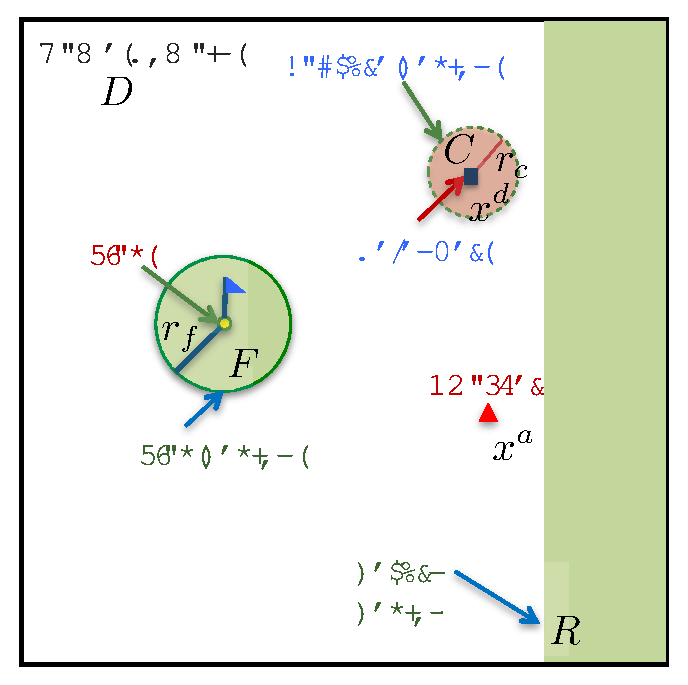
\includegraphics[width=0.9\columnwidth]{figures/gameDiagram}
	\caption{\textbf{The basic configuration of the capture-the-flag game.}}
	\label{fig:gameDiagram}
\end{figure}

The playing domain is assumed to be some rectangular set $D \subset \R^2$. The ``safe'' return region for the attacker is a rectangular strip $R \subset D$, and the flag is located in a circular region $F \subset D$ with radius $r_f$ (see Figure~\ref{fig:gameDiagram}). 

A configuration of the game is described by the vector $(x^a,x^d) \in \mathbb{R}^4$, where $x^a$ and $x^d$ are the planar positions of the attacker and defender, respectively. As per the rules of the game, the defender is constrained to remain outside of the flag and return regions, while the attacker can move freely through either. Thus, the set of permissible configurations is given by $\hat{D} = D \times D \setminus (F \cup R) \subset \R^4$. The equations of motion are given by $\dot{x}^a = u$ and $\dot{x}^d = d$, where $u$ and $d$ are the velocity inputs, constrained by speed limits $V_{a,max}$ and $V_{d,max}$ according to  $|| u ||_2 \leq V_{a,max}$ and $|| d ||_2 \leq V_{d,max}$. For fairness, we assume that $V_{a,max} = V_{d, max}$.  The attacker is considered to be tagged or intercepted by the defender if the defender comes within distance $r_c$ of the attacker. This corresponds to a capture region $C = \left\{ (x^a,\ x^d) \in \mathbb{R}^4:  ||x^a - x^d||_2 \leq r_c\right\}$.

Victory for the attacking player is attained by meeting all of the following conditions, assuming the game takes place over some finite time horizon $[0, T_f]$:
\begin{itemize}
\item{Flag capture: $x^a(T_c) \in F$ for some finite time $T_c$ where $0 \leq T_c \leq T_f$ }
\item{Flag return:  $x^a(T_r) \in R$ for some finite time $T_r $ where $T_c \leq T_r \leq T_f$}
\item{Avoiding defender capture: \\
$x^a(t) \in D \bigwedge (x^a(t), x^d(t)) \not \in C$ for all time $t \in [0, T_r] $} 
\end{itemize}
Victory for the defending player is achieved by preventing the attacker from achieving any of the above conditions by $T_f$ while obeying the constraint $x^d \in D \setminus (F \cup R)$. It should be remarked that when $T_f$ is small, the options of the attacking player may be severely restricted by the time limit. Correspondingly, this also leads to simplistic delaying strategies by the defending player. Motivated by this consideration, we will be specifically interested in scenarios where $T_f$ is large, namely as $T_f$ approaches $\infty$.

It is assumed that the positions of both players are fully observable to each other, and that the defender input $d(t)$ may be a function of the attacker input $u(t)$ at each time $t$. The latter assumption corresponds to a choice in the order of play to prevent an infinite regression of second-guessing between the players. For the simple dynamics considered here, the opposite order of play leads to an equivalent problem formulation and identical solutions.

The goal of this work is to provide a solution to this two-player game of capture-the-flag in terms of both the winning regions and winning strategies for each player. For the attacker, we would like to determine a subset of initial configurations $W_A \subset \mathbb{R}^4$ for which there exists a feasible attacker control strategy for achieving the victory conditions, regardless of the control strategy of the defending player. Furthermore, for any configuration in $W_A$, we would like to determine a winning strategy that ensures the attacker objectives. Clearly, for any permissible initial configuration outside this set, there exists some defender strategy so as to prevent the attacker from achieving victory, regardless of the attacker strategy. Thus, the defender winning set $W_D$ is given simply as $\hat{D} \setminus W_A$. 

In building up towards the full winning sets, we will also characterize the partial winning sets for the flag capture and flag return phases of the game. Some useful terminologies are summarized below.
\begin{itemize}
\item{{\bf Flag Capture Set $F_A$}: configurations from which the attacker can achieve flag capture while avoiding defender interception.}
\item{ {\bf Stop Capture Set $F_D$}: $\hat{D} \setminus F_A$, where the defender can prevent flag capture by the attacker.}
\item{ {\bf Flag Return Set $R_A$}: configurations from which the attacker can achieve flag return while avoiding defender interception.} 
\item{ {\bf Stop Return Set $R_D$}: $\hat{D} \setminus R_A$, where the defender can prevent flag return by the attacker.}
\end{itemize}

%%%%%%%%%%%%%%%%%%%%%%%%%%%%%%%%%%%%%%%%%%%%%%%%%%%%%%%%%%%%%%%%%%%%%%%%%%%%%%%%
%%%%%%%%%%%%%%%%%%%%%%%%%%%%%%%%%%%%%%%%%%%%%%%%%%%%%%%%%%%%%%%%%%%%%%%%%%%%%%%%
\section{Hamilton-Jacobi Reachability in Capture-the-Flag}
\label{sec:hj_formulation}
Capture-the-flag falls naturally under the framework of differential games due to the competing objectives of the attacking and defending players~\cite{b:basar-olsder-1999}. This allows us to characterize the winning regions of the attacker and defender from the results of numerical Hamilton-Jacobi reachable set calculations~\cite{j:mitchell-TAC-2005,mitchell-thesis}.

The numerical Hamilton-Jacobi approach has a number of advantages. Although it is possible to use geometric analysis to construct some solutions to the game for simple configurations of the game regions, the numerical approach allows arbitrarily complex geometries to be addressed, including obstacles. Moreover, this framework naturally allows for the sequential aspect of the game, where the attacker must first reach the flag zone and then subsequently return to safety. Such sequencing is very difficult to analyze otherwise.  

As a further benefit, we can derive approximate winning control strategies for the respective players from the solutions of these computations. For details on the theoretical background behind the application of Hamilton-Jacobi equations to problems in optimal control and differential games, the interested reader is referred to~\cite{b:bardi-1997}. 

\subsection{Hamilton-Jacobi Reachability}
\label{subsec:hj_background}
We refer to the two players in a general differential game as Player I and Player II. We assume that the continuous dynamics are modeled by the ordinary differential equation 
\begin{equation}
\label{eq:dynamics}
\dot{x} = f(x, u, d), \ x(0) = x_0
\end{equation}
where $x \in \mathbb{R}^n$ is the system state,  $u$ is the control input of Player I, $d$ is the control input of Player II, and $x_0$ is the initial condition. The input ranges of Player I and Player II will be denoted by $\mathbb{U}$ and $\mathbb{D}$, respectively. 

In terms of control strategies, Player I selects controls $u(t), t \in [0,T]$, satisfying $u(t) \in \mathbb{U}$, possibly as a function of the state $x(t)$. Similarly, Player II selects controls $d(t), t \in [0,T]$, satisfying $d(t) \in \mathbb{D}$. However, we allow this selection to be a function of both the state $x(t)$
and the control $u(t)$ of Player I. The set of permissible control strategies for Players I and II are denoted by $P(T)$ and $\Gamma(T)$, respectively.

Now consider sets $R, A \subset \mathbb{R}^n$ and time horizon $[0, T]$, we are interested in computing the set of initial conditions $x_0 \in \mathbb{R}^n$ for which there exists some choice of Player I control policy $\pi(T) \in P(T)$, such that regardless of the choice of Player II control strategy $\gamma(T) \in \Gamma(T)$, the state trajectory $x(\cdot)$ under model (\ref{eq:dynamics}) satisfies $x(t) \in R$ for some $t \in [0,T]$ and $x(s) \notin A$, $\forall s \in [0,t]$. In other words, this is the set of initial conditions that can be controlled into $R$ within finite time by Player I, while avoiding $A$ at all times, regardless of the control strategy of Player II. We denote this set by $\mathcal{RA}_T(R,A)$, and refer to it as the \emph{reach-avoid} set over $[0,T]$.

Under suitable conditions, given in~\cite{j:mitchell-TAC-2005} and~\cite{mitchell-thesis}, the reach-avoid set can be obtained from the solution of a constrained Hamilton-Jacobi-Isaacs (HJI) partial differential equation (PDE), using level set representation of sets. Under this representation, a set $G \subset \mathbb{R}^n$ is defined implicitly as the sublevel set of a function $\phi_G: \mathbb{R}^n \rightarrow \mathbb{R}$, such that $G = \left\{x\in \mathbb{R}^n, \phi_G (x) \leq 0\right\}$.

Let $\phi: \mathbb{R}^n \times [-T,0] \rightarrow \mathbb{R}$ be the viscosity solution~\cite{j:Crandall-TAMS-1983} of the following constrained terminal value HJI PDE,
\begin{equation}
	\label{eq:HJ_PDE_reachavoid}
	\frac{\partial \phi}{\partial t} + \min \left[0, H\left(x,\frac{\partial \phi}{\partial x}\right)\right] = 0,\;\phi(x,0) = \phi_R(x)	 
\end{equation}
subject to 
$$\phi(x,t) \geq -\phi_A(x)$$
where the optimal Hamiltonian is given by
$$H\left(x,p\right) = \min_{u \in \mathbb{U}} \max_{d \in \mathbb{D}} p^T f(x,u,d)$$
and $\phi_R, \phi_A$ are the level set representations of $R$ and $A$, respectively.  Then by the argument presented in~\cite{j:mitchell-TAC-2005} and~\cite{mitchell-thesis}, the reach-avoid set is given by 
$$\mathcal{RA}_T(R,A) = \left\{x\in \mathbb{R}^n, \phi (x,-T) \leq 0\right\}$$
A highly accurate numerical solution to equation (\ref{eq:HJ_PDE_reachavoid}) can be computed using the Level Set Toolbox for MATLAB~\cite{LSToolbox}.

\subsection{Reachability for Capture-the-Flag}
%The capture-the-flag problem can be solved using a sequence of two reach-avoid calculations. The general idea is as follows. First we calculate the set of states in the joint state space from which the attacker can reach base $R$ after reaching flag $F$ while avoiding capture and staying inside domain $D$. This gives us the set of winning configurations for the flag return phase of the game. The attacker victory set $W_A$ is then the set of initial conditions from which the attacker can reach one of these winning configurations while avoiding capture. 

In this section, we characterize the attacker victory sets $F_A$, $R_A$, and $W_A$ using the reach-avoid operator. The corresponding defender victory sets $F_D$, $R_D$, and $W_D$ can be obtained via the relations described in Section~\ref{sec:formulation}. Under the differential game setting, the attacker takes on the role of Player I, while defender takes on the role of Player II.  

We first consider the flag return phase of the game, taking place over some time horizon $[0,T_r]$. The goal of the attacker during this phase is to arrive in the return region $R$ within $[0,T_r]$, while avoiding capture by the defender. The rules require both players to stay within the game region $D$ and the defender to remain outside of $F$ and $R$. In the framework of a differential game, we encode the constraints for each player as part of the winning conditions for the other, so that the attacker wins if the defender violates its constraints and vice versa. Note that this formulation can also be used to encode other state constraints such as obstacles. 

Let $x$ be the joint configuration $(x^a, x^d)$, $D^C$ the complement of $D$ in $\mathbb{R}^2$, and $G_A = \left\{x \in \mathbb{R}^4: x^a \in D^C \right\}$, then the attacker winning condition are $O_R \vee O_D$, where
\begin{align*}
&O_R = \left\{\exists t \in [0,T_r], x^a(t) \in R \wedge x(s) \notin C \cup G_A, \forall s \in [0,t]\right\} \\
&O_D = \left\{\exists t \in [0,T_r], x^d(t) \in F \cup R \cup D^C \wedge x(s) \notin C \cup G_A, \right. \\
&\left. \forall s \in [0,t]\right\}
\end{align*}
Define the sets $G_D = \left\{x \in \mathbb{R}^4: x^d \in F \cup R \cup D^C \right\}$ and $G_R = \left\{x \in \mathbb{R}^4: x^a \in R \right\}$. Then from the above conditions, we can compute the flag return set as
\begin{equation}
R_A = \mathcal{RA}_{T_r}(G_R \cup G_D, C \cup G_A)
\end{equation}

Now consider the flag capture phase of the game, with a time horizon of $[0,T_c]$. If the second phase of the game is ignored, then the goal of the attacker is to simply arrive in the flag region $F$ within $[0,T_c]$ while avoiding interception by the defender, and the goal of the defender is to intercept the attacker or prevent the attacker from reaching $F$. Using the same constraint encoding as before, the attacker winning condition for this phase is given by
$O_F \vee O_D$, where
\begin{align*}
&O_F = \left\{\exists t \in [0,T_c], x^a(t) \in F \wedge x(s) \notin C \cup G_A, \forall s \in [0,t]\right\} 
\end{align*}
Define the set $G_F = \left\{x \in \mathbb{R}^4: x^a \in F \right\}$. Then the flag capture set can be computed as
\begin{equation}
F_A = \mathcal{RA}_{T_c}(G_F \cup G_D, C \cup G_A)
\end{equation}

However, when both phases of the game are considered, it is clearly insufficient for the attacker to simply arrive in $F$. If the defender chooses a strategy such that the attacker arrives at the flag but the overall state $(x^a, x^d)$ is in a configuration outside the flag return set $R_A$, then the defender can prevent the attacker from returning safely to $R$. In order to ensure flag return, the attacker must reach the set of configurations $\tilde{R}_A = G_F \cap R_A$ during the first phase of the game. This corresponds to the modified attacker objectives during the flag capture phase $\tilde{O}_F \vee O_D$, where
\begin{align*}
\tilde{O}_F\! =\!\left\{\exists t \in \![0,T_c], x(t) \!\in \!\tilde{R}_A \wedge x(s)\! \notin \!C \cup G_A, \forall s \in [0,t]\right\}
\end{align*}
From this, we can compute the attacker winning set as
\begin{equation}
W_A = \mathcal{RA}_{T_c}(\tilde{R}_A \cup G_D, C \cup G_A)
\end{equation}

\subsection{Control Strategies}
\label{sub:ctrl_inputs}
Based upon the approach described in~\cite{j:Lygeros-automatica-1999} and~\cite{j:Tomlin-ProcIEEE-2000}, we describe here a method for the synthesis of winning strategies in regions of the state space where the solution $\phi$ to~(\ref{eq:HJ_PDE_reachavoid}) is differentiable.  For pursuit-evasion games, the solution to the HJI equation is typically differentiable away from some singular surfaces where the winning strategies are not uniquely defined~\cite{b:basar-olsder-1999}.  With arbitrarily small perturbations from these surfaces, the solution becomes differentiable, allowing application of the techniques described here.  

Under this setting, for $x \in \mathcal{RA}_T(R,A)$, the control strategy that allows Player I to achieve the desired objectives regardless of the control strategy of Player II is described by
\begin{equation}
	\label{eq:opt_ctrl_u}
  u^*(x,t)\! =\! \arg \min_{u \in \mathbb{U}} \max_{d \in \mathbb{D}} p(x,-t)^T f(x,u,d), \!\ t \in [0,T] 
\end{equation}
where $p = \frac{\partial \phi}{\partial x}$.  Similarly, for $x \notin \mathcal{RA}_T(R,A)$, the Player II control strategy that is guaranteed to prevent Player I from achieving the desired objectives is given by
\begin{equation}
	\label{eq:opt_ctrl_d}
  d^*(x,t) = \arg \max_{d \in \mathbb{D}} p(x,-t)^T f(x,u^*,d), \ t \in [0,T] 
\end{equation}
Given the numerical computation of the set $\mathcal{RA}_T(R,A)$, the derivatives of $\phi$ are not available in closed form.  Nonetheless, approximate control laws can be obtained by temporal discretization, for example at sampling instants $kT, k = 0,1,...$, and computing numerical derivatives of $\phi(x,-kT)$. 

For the capture-the-flag problem, the optimal Hamiltonian is given by
$$H\left(x,p\right) = \min_{u \in \mathbb{U}} \max_{d \in \mathbb{D}} p_u^T u + p_d^T d$$
where $p_u = (p_1, p_2)$ and $p_d = (p_3, p_4)$. From this we can deduce the explicit winning strategies\footnote {The choice of player order does not affect the player strategies in this problem because the optimal defender and attacker inputs are independent of each other.}
\begin{align}
	\label{eq:opt_ctf_u}
  u^*(x,t) &= -V_{a,max} \frac{p_u(x,-t)}{||p_u(x,-t)||_2} \\
	\label{eq:opt_ctf_d}
  d^*(x,t) &= V_{d,max} \frac{p_d(x,-t)}{||p_d(x,-t)||_2}
\end{align}

%Intuitively, this corresponds to moving at maximum allowable velocity along the directions indicated by the time-varying directional derivatives $-p_u(x(t),-t) \in \mathbb{R}^2$ or $p_d(x(t),-t) \in \mathbb{R}^2$.

Over short time horizons, time varying strategies can be synthesized for the flag capture and flag return phases of the game as per equations (\ref{eq:opt_ctf_u}) and (\ref{eq:opt_ctf_d}), using $W_A$ and $R_A$, respectively. Under the attacker control strategy constructed from $W_A$, the trajectory $x = (x^a, x^d)$ is guaranteed to enter $\tilde{R}_A$ within $[0,T_c]$, satisfying the flag capture objective. At the time instant when $x(t) \in \tilde{R}_A$, the attacker can switch to the control strategy constructed from $R_A$ and safely return to $R$, thus winning the game.

In certain cases where the solution to (\ref{eq:HJ_PDE_reachavoid}) converges, namely $\lim_{t \rightarrow -\infty} \phi(x,t) = \phi_\infty(x)$ for some $\phi_\infty: \mathbb{R}^n \rightarrow \mathbb{R}$, time-invariant control strategies approximating (\ref{eq:opt_ctrl_u}) and (\ref{eq:opt_ctrl_d}) can be constructed. Specifically, suppose $\phi$ is computed numerically at time steps $-kT_s, k = 0,1,...$, we can select an index $k_0$ at which $||\phi(\cdot, -k_0 T_s) - \phi(\cdot, -(k_0+1)T_s)||_\infty < \epsilon$, for some tolerance $\epsilon > 0$. If $\epsilon$ is chosen sufficiently small, we can reasonably assume that $\phi(\cdot, -t) \approx \phi(\cdot, -k_0 T_s)$, $\forall t > k_0 T_s$. This allows us to approximate the long-term strategies of the two players by
\begin{align}
	\label{eq:opt_ctrl_inf_u}
  u^*(x) &\approx \arg \min_{u \in \mathbb{U}} \max_{d \in \mathbb{D}} p(x,-k_0 T_s)^T f(x,u,d) \\
  \label{eq:opt_ctrl_inf_d}
  d^*(x) &\approx \arg \max_{d \in \mathbb{D}} p(x,-k_0 T_s)^T f(x,u^*,d) 
\end{align}

For our application, the sets $R_A$ and $W_A$ indeed converge numerically for sufficiently large $T_r$ and $T_c$, leading to approximate long-term strategies for the attacker and defender.


\begin{figure}[h]
	\centering
	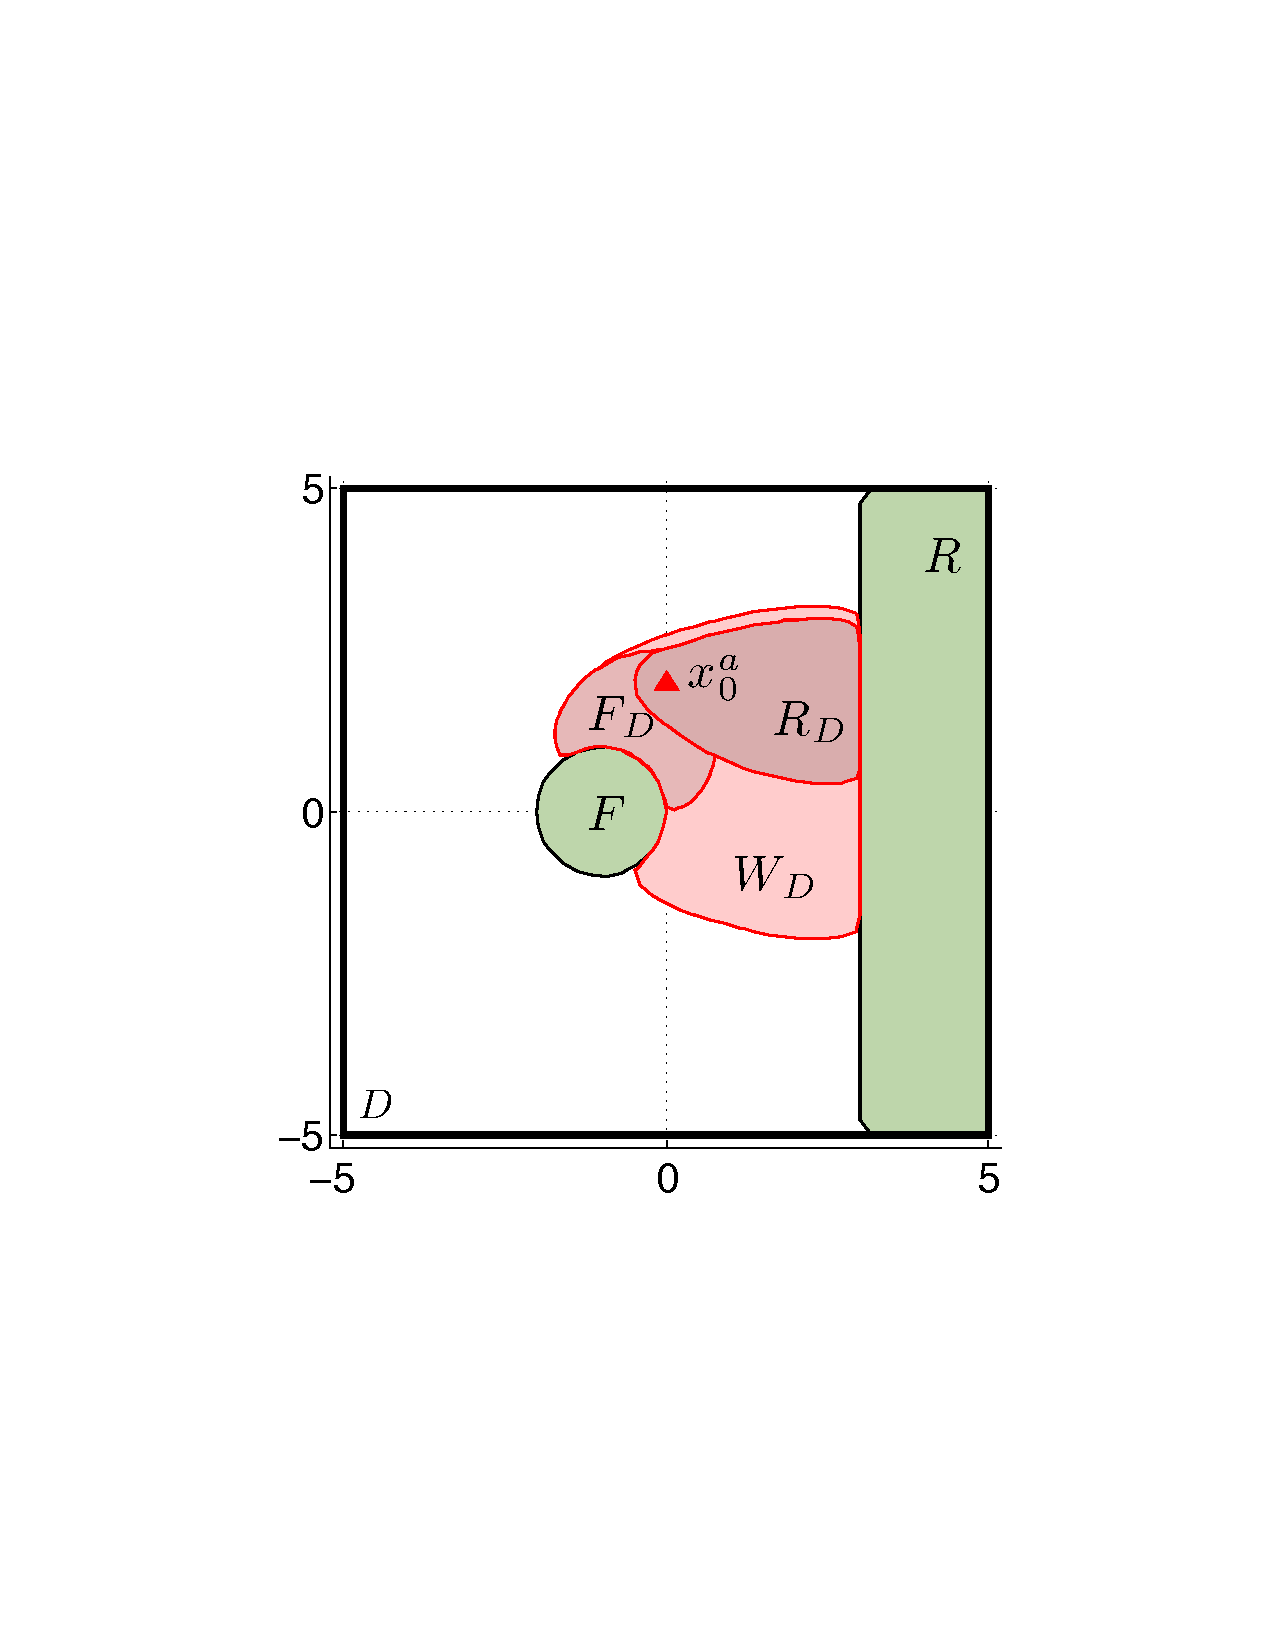
\includegraphics[width=0.6\columnwidth]{figures/FCFR45.pdf}
	\caption{\textbf{The overall winning region $W_D$ of the defender for $x^a = (2,2)$, with $R_D$ and $F_D$ super-imposed for comparison.}}
	\label{fig:defenderWinSet}
\end{figure}
%%%%%%%%%%%%%%%%%%%%%%%%%%%%%%%%%%%%%%%%%%%%%%%%%%%%%%%%%%%%%%%%%%%%%%%%%%%%%%%%
\section{Computational Results}
\label{sec:results}

%\begin{figure}[tb]
%	\centering
%\begin{tabular}{cc}
%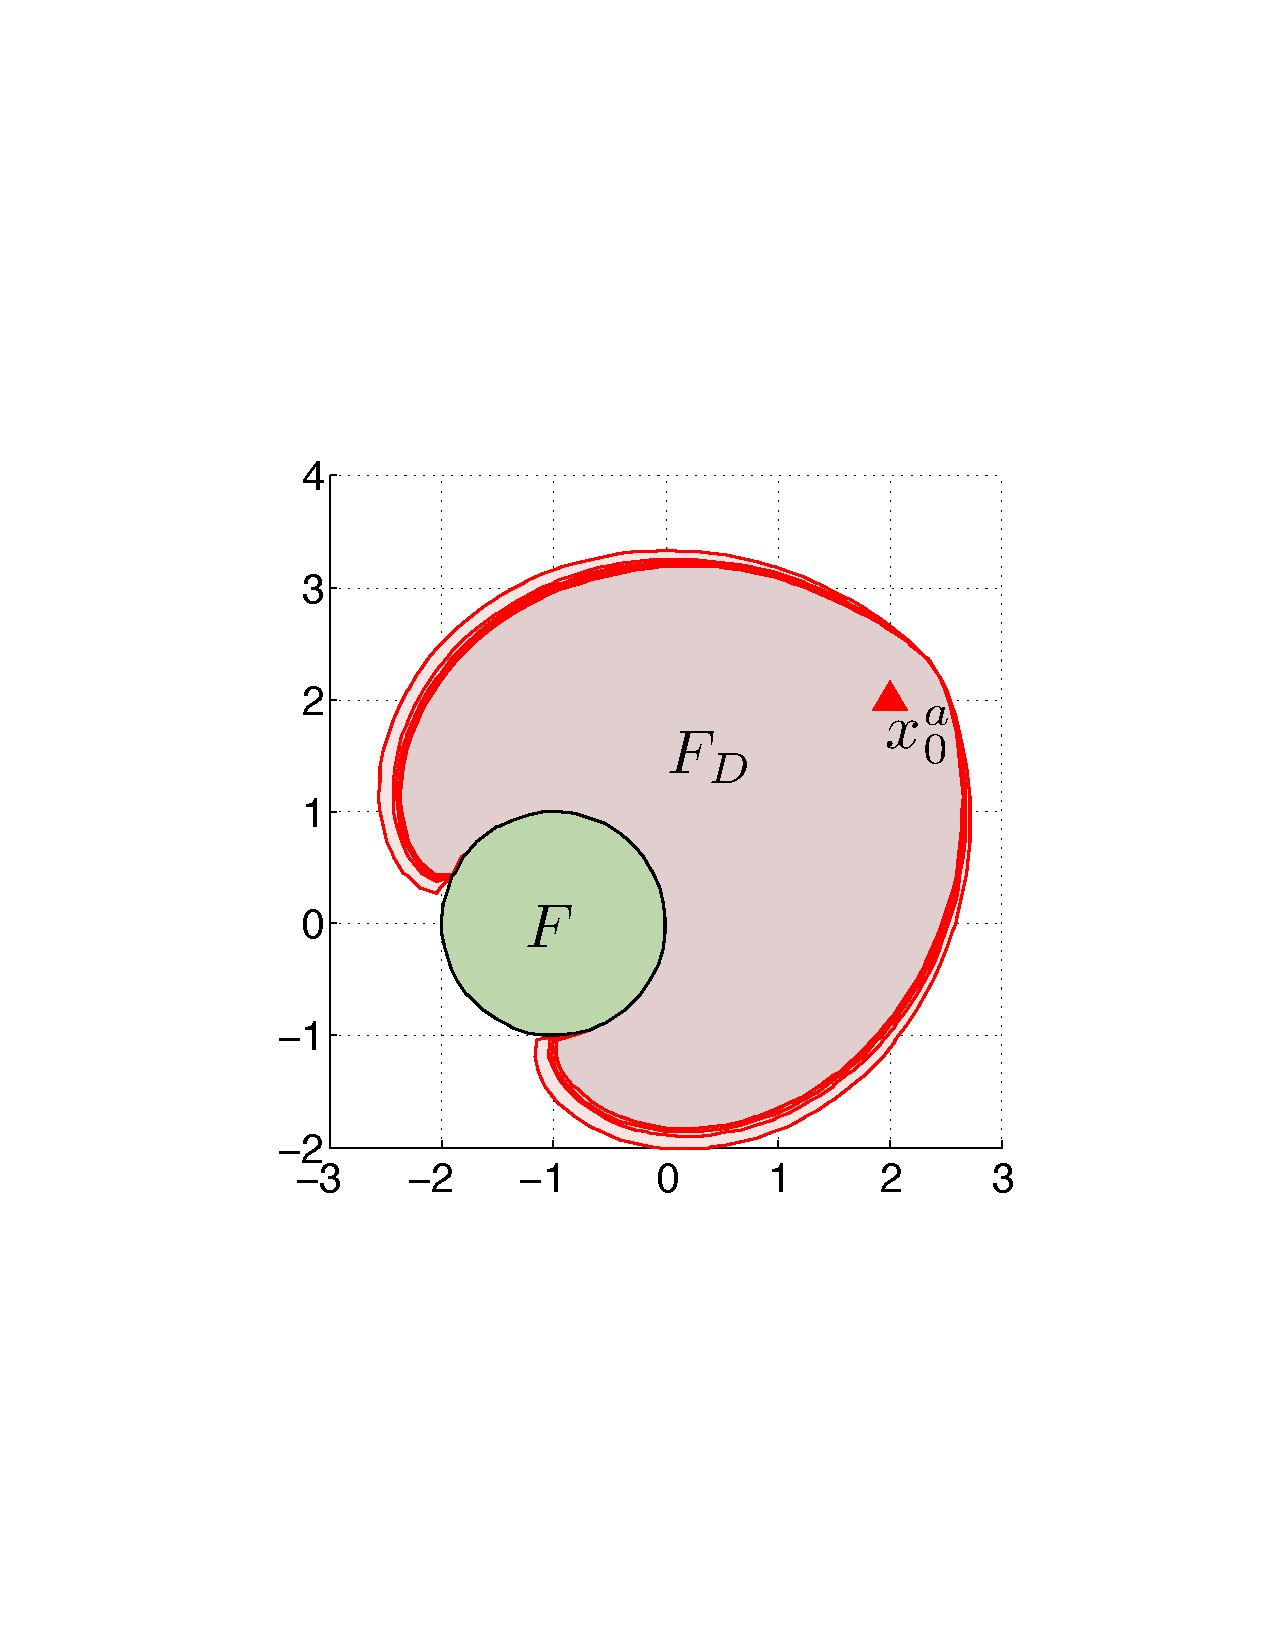
\includegraphics[width=0.45\linewidth]{figures/FC45.pdf} &
%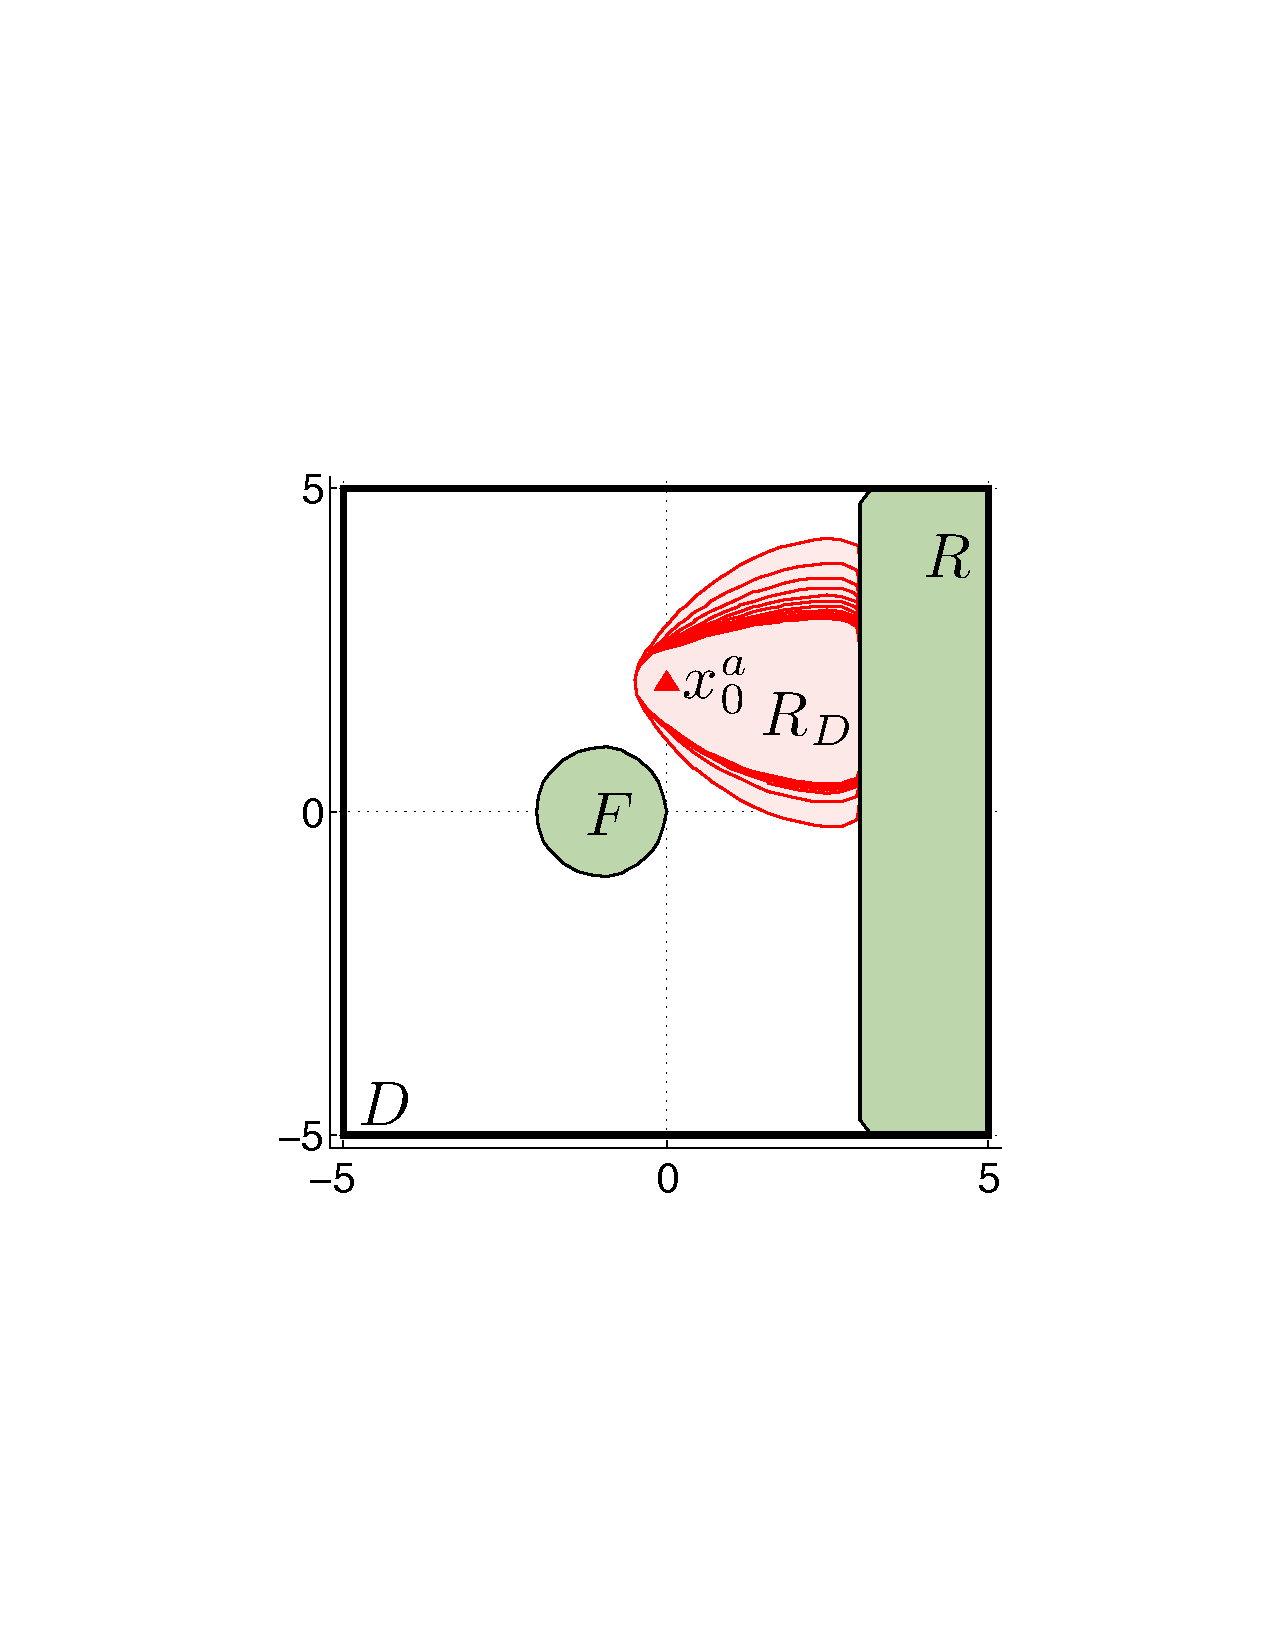
\includegraphics[width=0.45\linewidth]{figures/FR45.pdf} \\
%(a) & (b) \\
%\end{tabular}
%\caption{\textbf{Computationally derived reachable sets for $r_c = 0.5$ for (a) $F_D$ and (b) $R_D$ as slices in $\R^2$ for fixed $x^a$. Note the convergence over time of the computed sets.}}
%\label{fig:compareBothResults}
%\end{figure}


\setlength\tabcolsep{0.5pt}
\begin{figure*}
	\centering
	\begin{tabular}{cccc}
		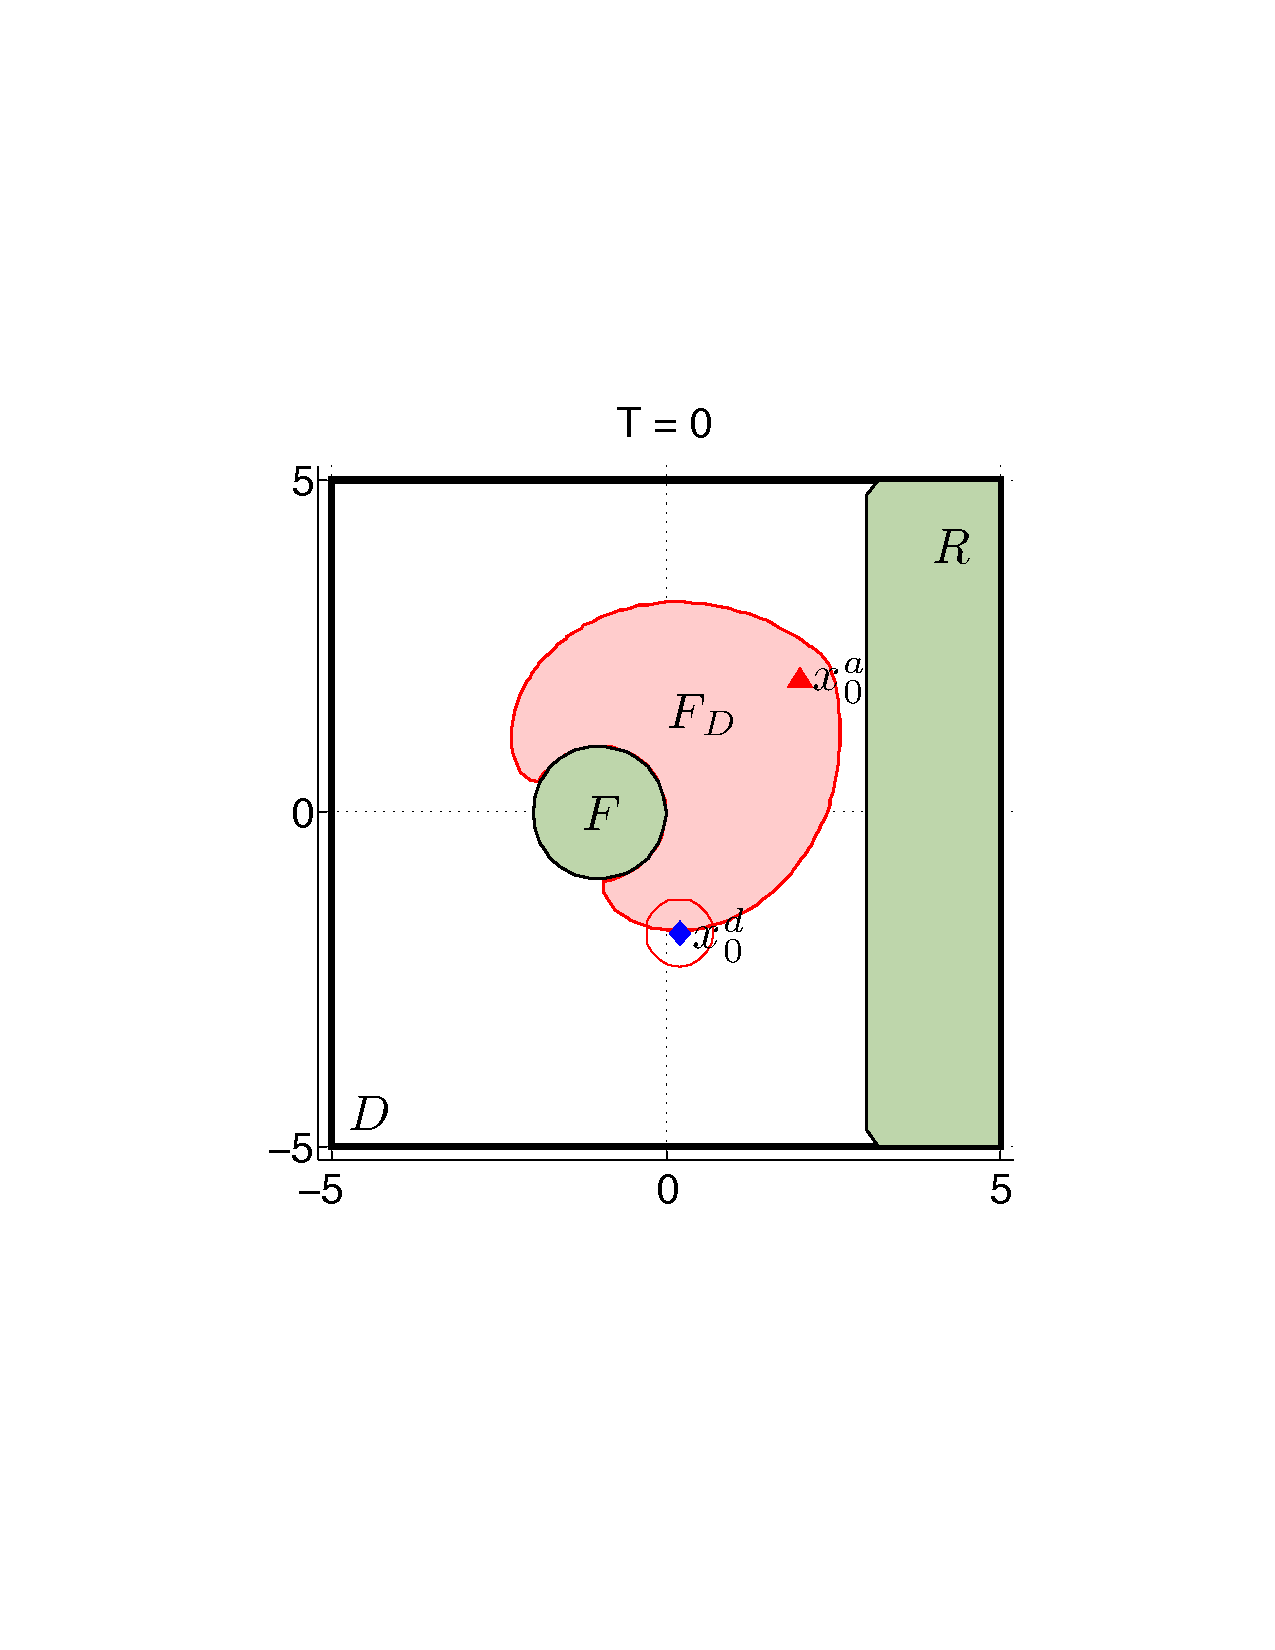
\includegraphics[width=0.25\textwidth]{figures/defenderWinFC/defenderWinFC1.pdf} &
		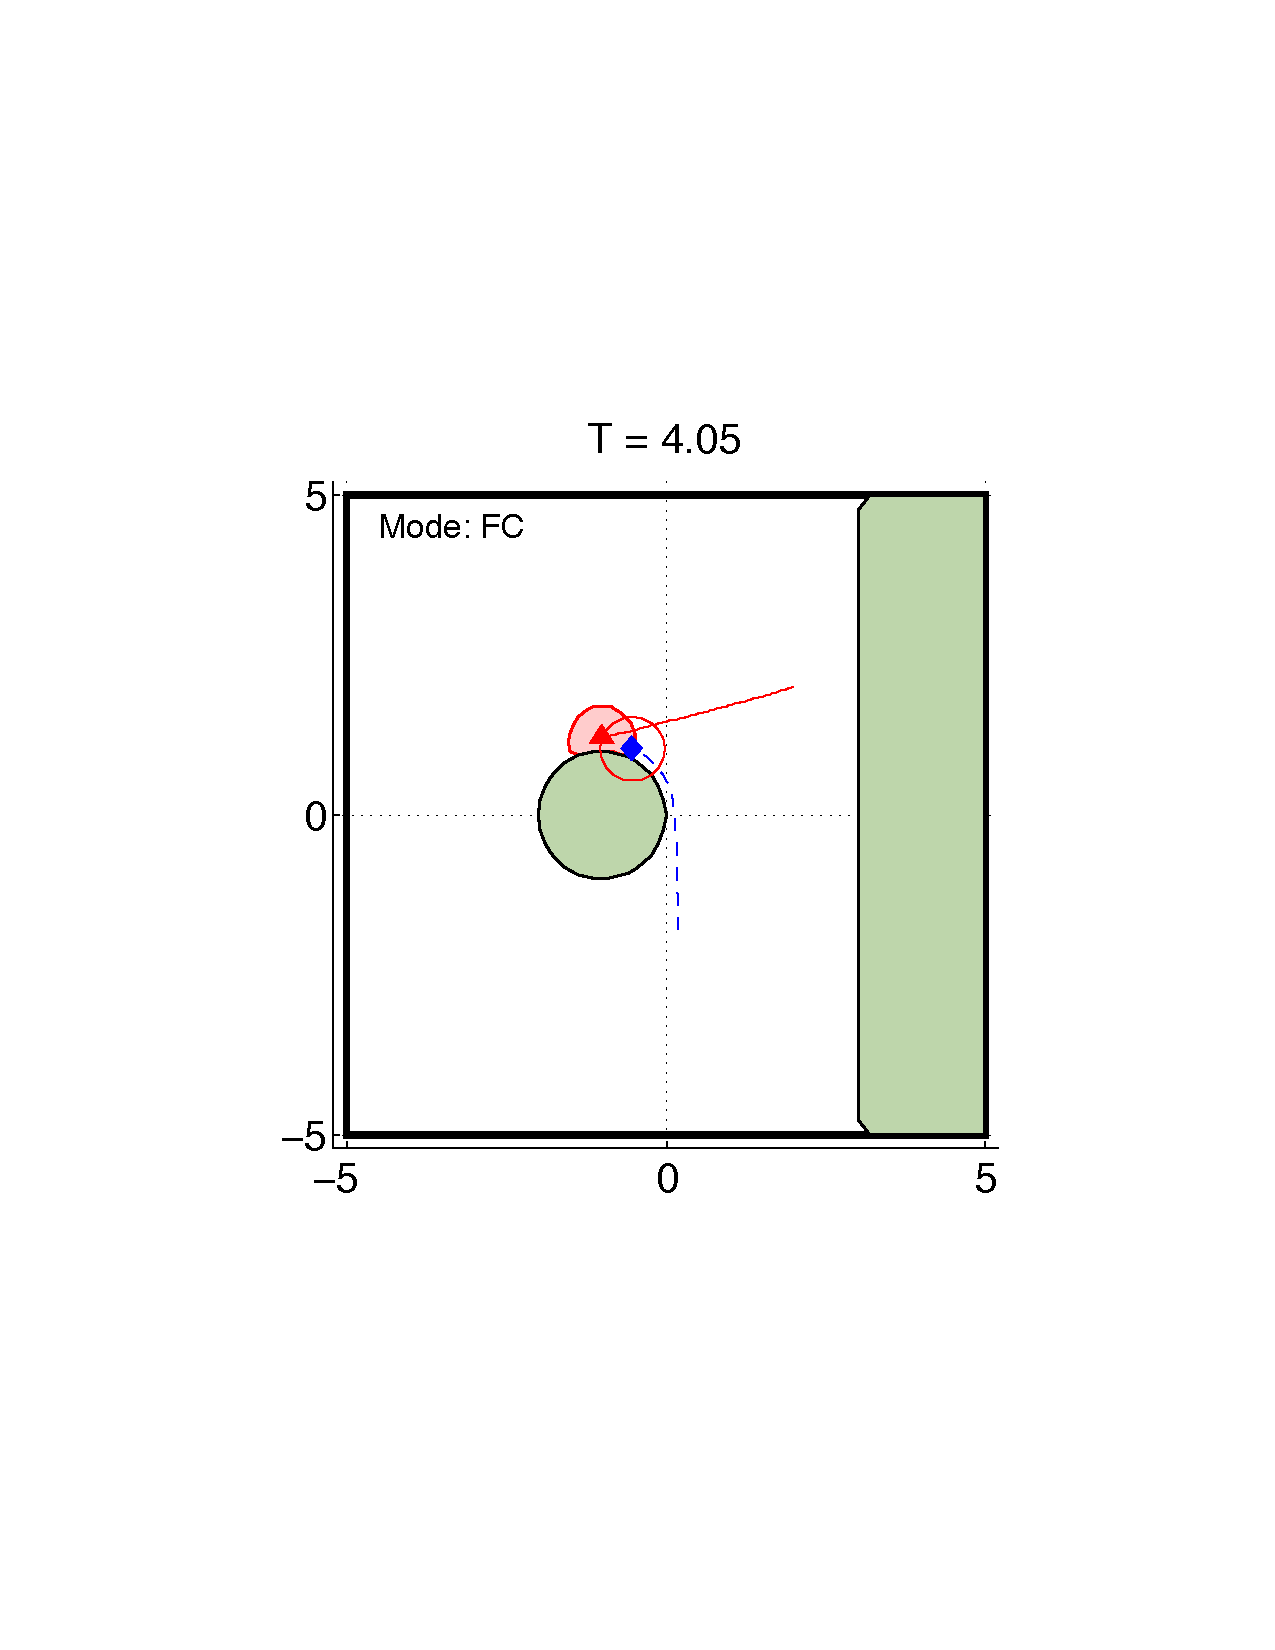
\includegraphics[width=0.25\textwidth]{figures/defenderWinFC/defenderWinFC7.pdf} &
		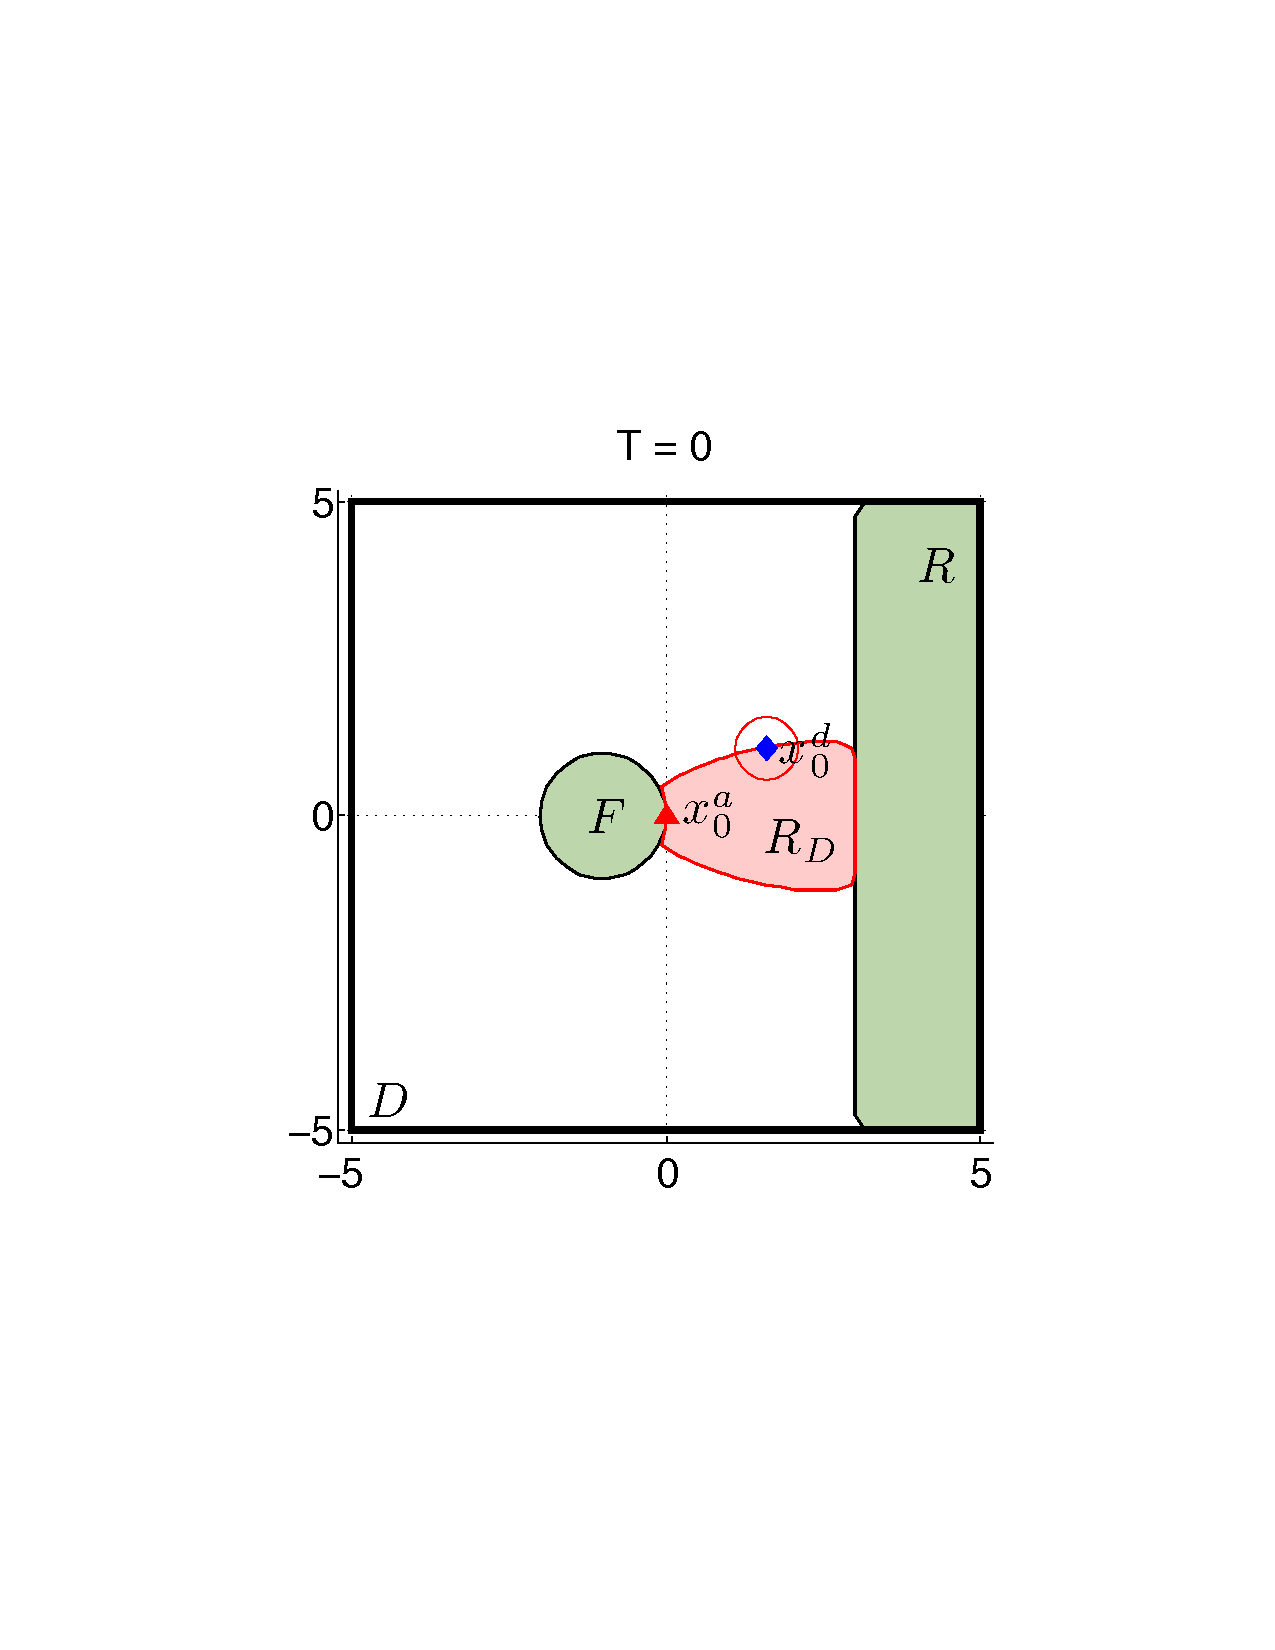
\includegraphics[width=0.25\textwidth]{figures/defenderWinFR/defenderWinFR1.pdf} &
		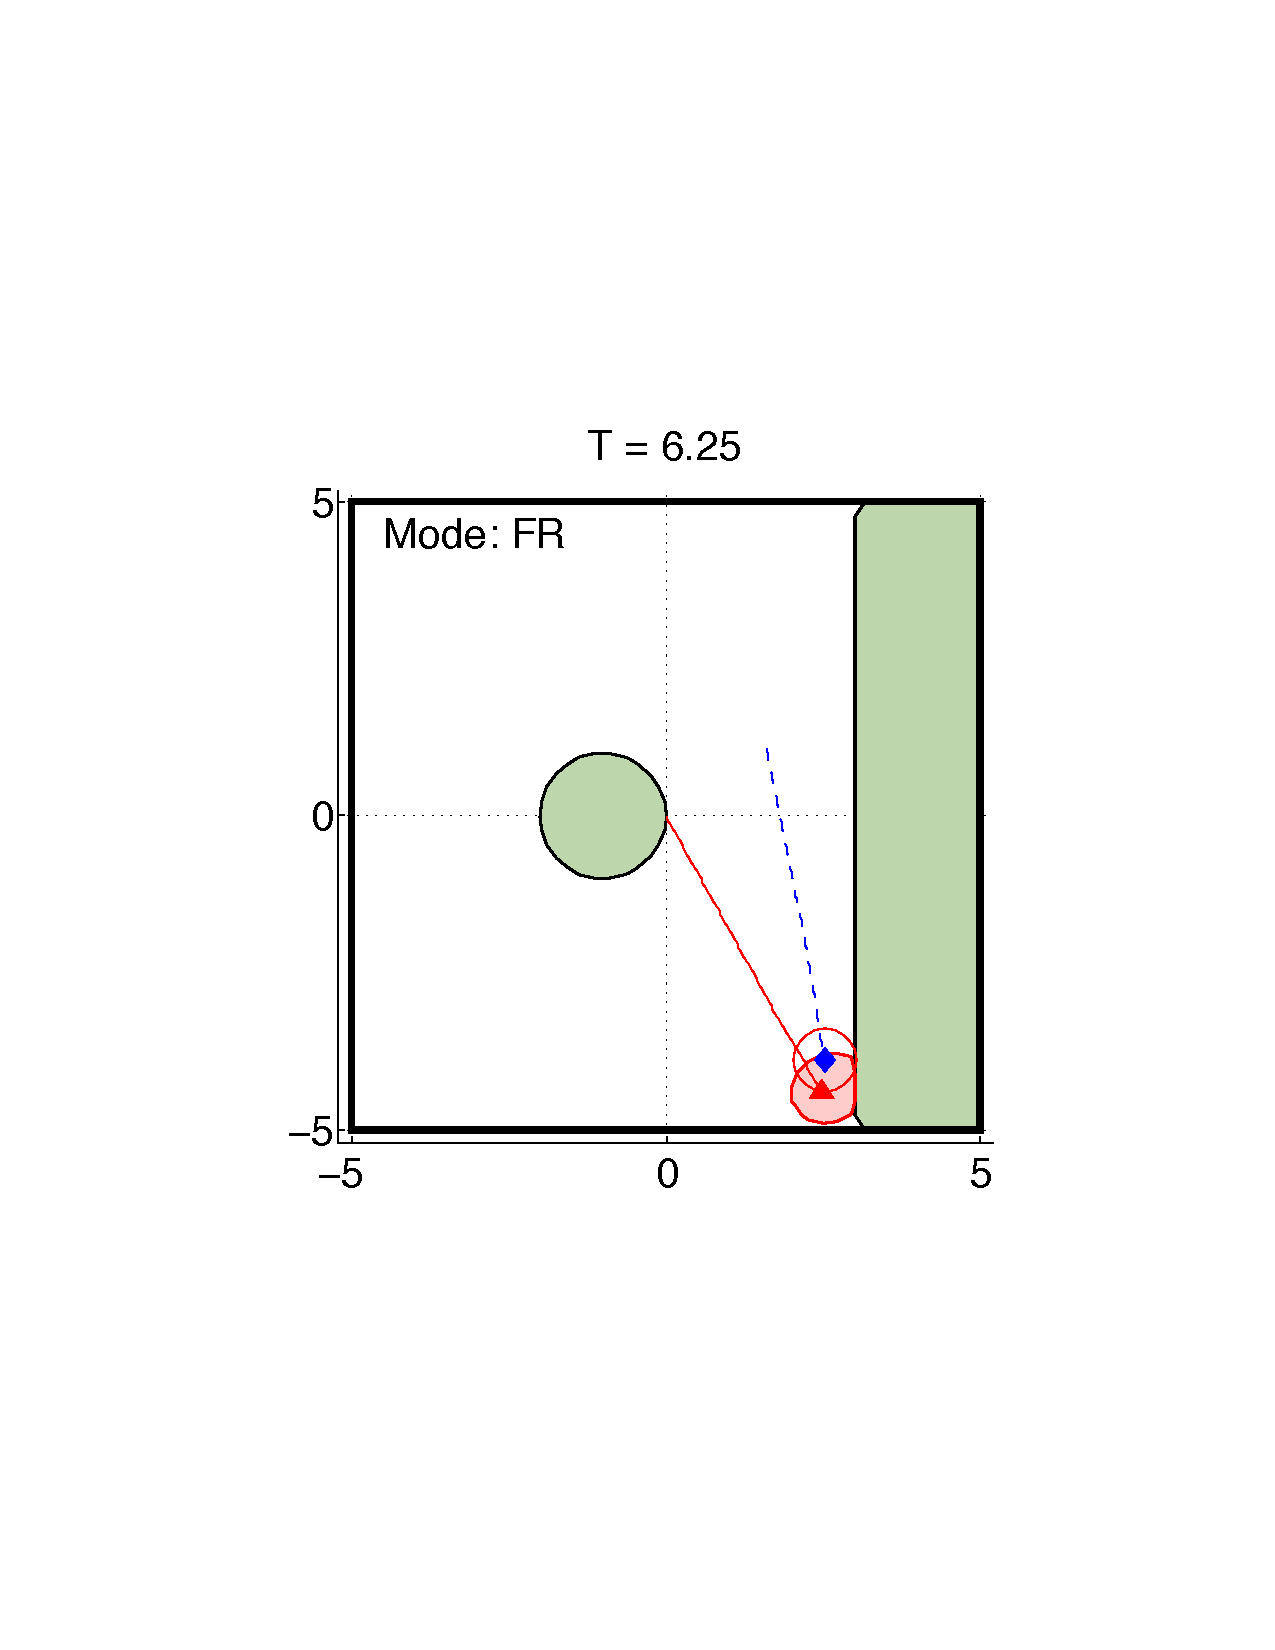
\includegraphics[width=0.25\textwidth]{figures/defenderWinFR/defenderWinFR4.pdf} \\
		(a) & (b) & (c) & (d)  \\
	\end{tabular} 
	\caption{\textbf{Two simulations showing cases where the defender (blue diamond) successfully intercepts the attacker (red triangle). (a) shows a scenario for flag capture only, with the resulting trajectories shown in (b). (c) and (d) show a similar scenario for flag return.}}
	\label{fig:defenderWin}
\end{figure*} 
\setlength\tabcolsep{6pt}

\setlength\tabcolsep{0.5pt}
\begin{figure*}
	\centering
	\begin{tabular}{cccc}
		\includegraphics[width=0.25\textwidth]{figures/defenderWinFCFR/defenderWinFCFR1.pdf} &
		\includegraphics[width=0.25\textwidth]{figures/defenderWinFCFR/defenderWinFCFR2.pdf} &
		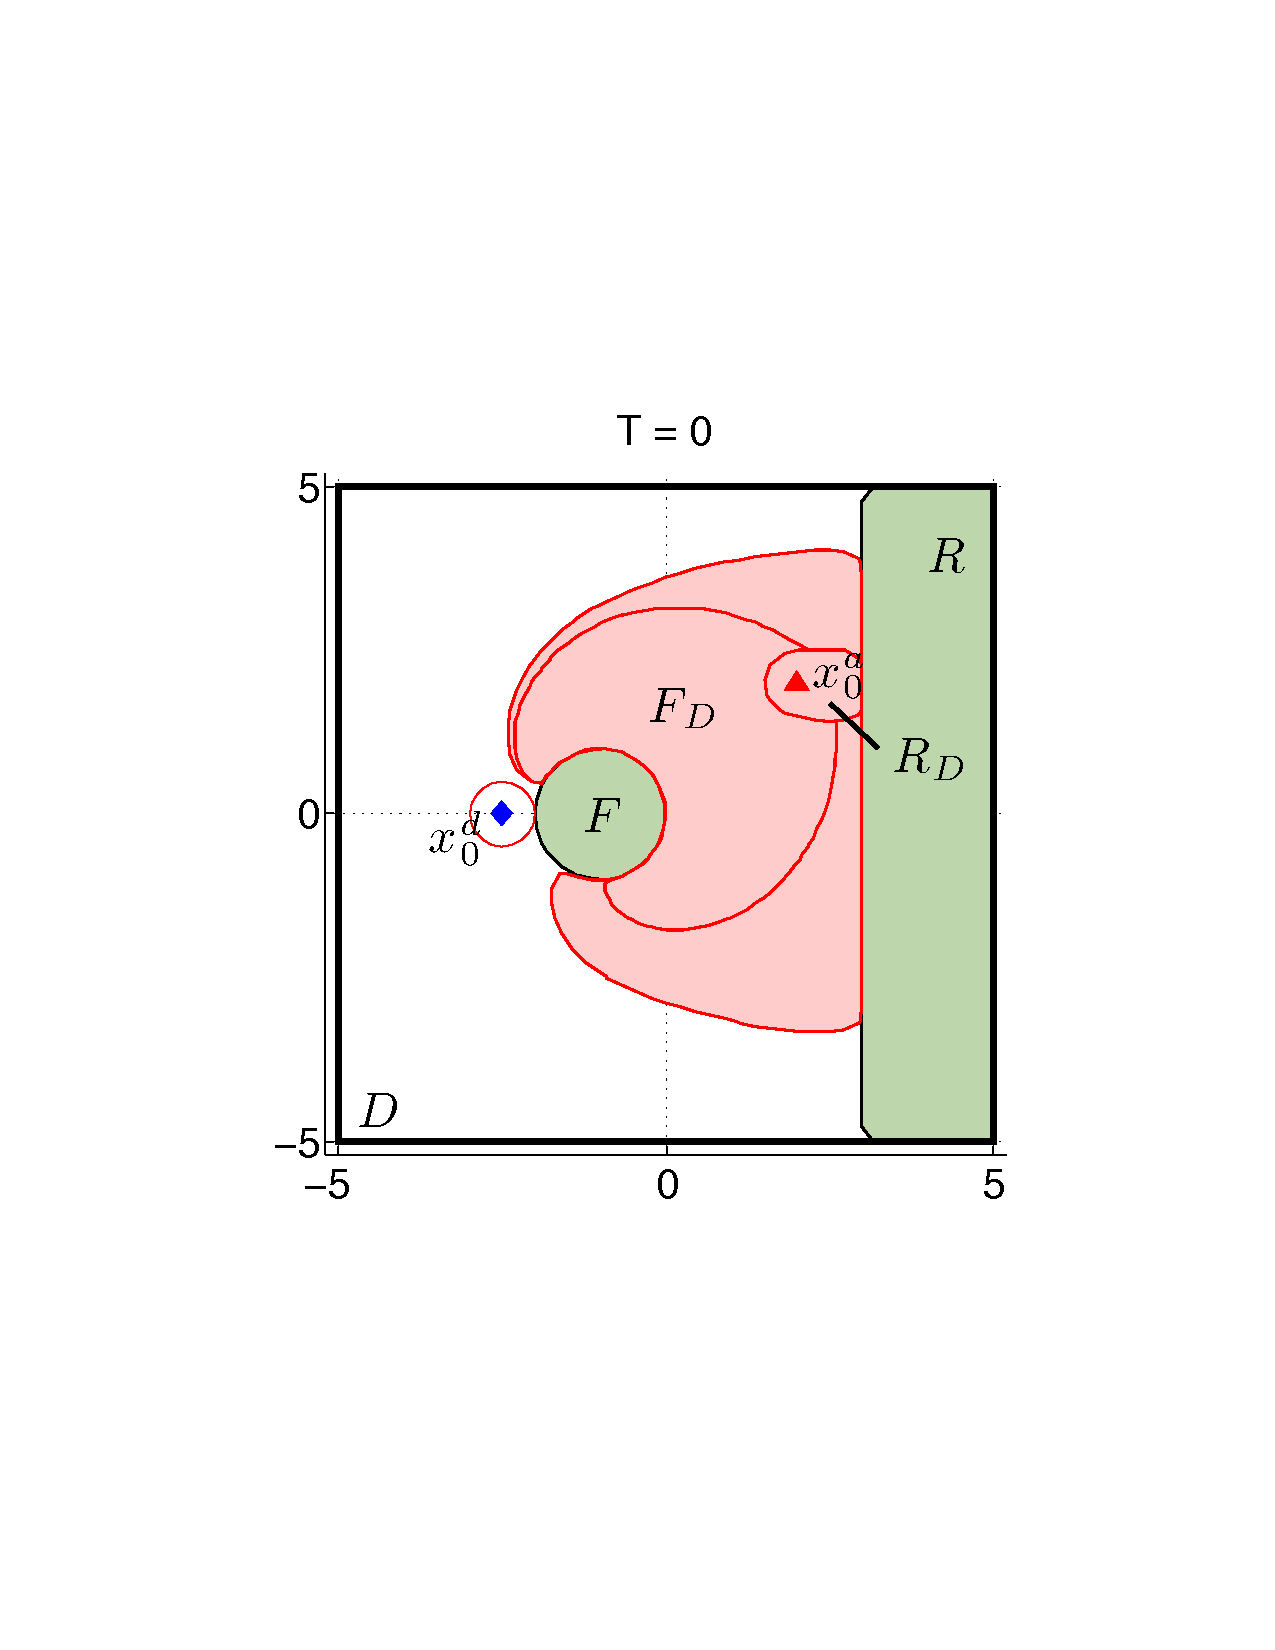
\includegraphics[width=0.25\textwidth]{figures/attackerWinFCFR/attackerwinFCFR1.pdf} &
		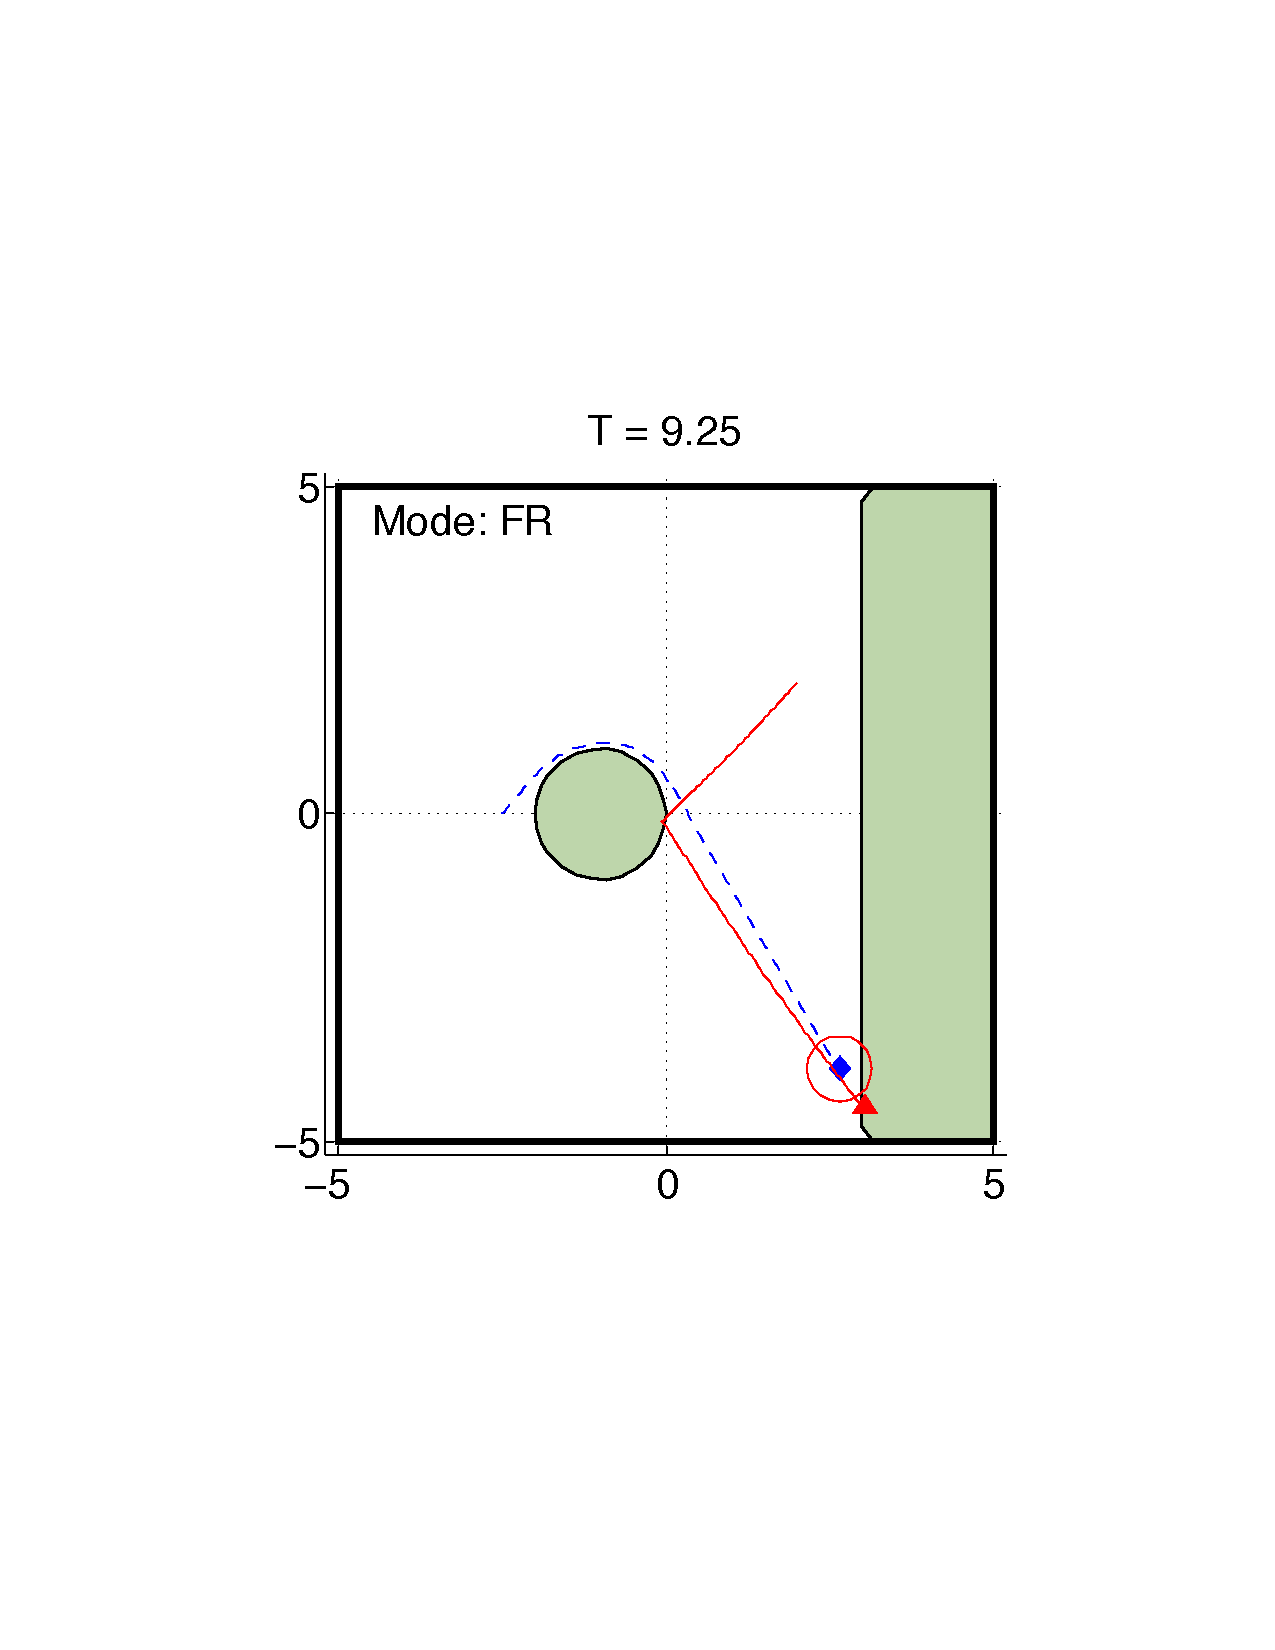
\includegraphics[width=0.25\textwidth]{figures/attackerWinFCFR/attackerwinFCFR2.pdf}\\
		(a) & (b) & (c) & (d)  \\
	\end{tabular} 
	\caption{\textbf{Two scenarios showing combined winning regions $W_D$ for both game modes. In (a) the defender starts inside $W_D$ and successfully prevents the attacker from returning with the flag, as seen in (b). (c) shows a case where the defender is outside of $W_D$, and is unable to prevent the attacker's successful flag capture and return, as shown in (d). }}
	\label{fig:combined}
\end{figure*} 
\setlength\tabcolsep{6pt}

The proposed reachability-based approach is illustrated through an example with $V_{a,max}=V_{d,max}=1$, $r_f = 1$, $r_c = 0.5$, and $T_f = 12$. The Hamilton-Jacobi reachable sets are calculated using the Level-Set Toolbox~\cite{LSToolbox} developed at the University of British Columbia. For the particular set of parameters, the sets  $F_D$, $R_D$ and $W_D$ all converge to fixed points after about 6 time units, corresponding to configurations from which the defender can always prevent the attacker from achieving the desired objectives, regardless of the time horizon. The actual sets lie in the 4-D joint configuration space $(x^a,x^d)$, but for visualization purpose, slices are shown in 2-D with $x^a$ fixed. For example, the converged sets $F_D$, $R_D$ and $W_D$ are shown in Figure~\ref{fig:defenderWinSet} with the attacker fixed at $(2,2)$ . It is observed that $W_D$ is much larger than simply $F_D \cup R_D$, reflecting strategies where the defender uses the time during the flag capture phase to arrive at a configuration that blocks the attacker's return path.

Using the reachable sets, simulations are conducted where the attacker and defender choose controls according to the strategies discussed in Section~\ref{sub:ctrl_inputs}. Figure~\ref{fig:defenderWin} shows two example scenarios, one for the flag capture phase and the other for the flag return phase. In both cases, the defender starts within the winning set and successfully intercepts the attacker. More interesting scenarios involving the interplay between the flag capture and flag return phase are demonstrated in Figure~\ref{fig:combined}. In Figure~\ref{fig:combined}a, the defender starts within the overall winning set $W_D$, but outside the set $F_D$. The trajectory simulation in Figure~\ref{fig:combined}b shows that the defender does not try to prevent flag capture. Instead it uses the time it takes for the attacker to reach the flag to get into position to prevent flag return, thereby winning the game. On the other hand, when the defender begins outside $W_D$, as in Figure~\ref{fig:combined}c, the simulated trajectory in Figure~\ref{fig:combined}d shows that the attacker is able to successfully capture the flag and return to the safe region, without being intercepted by the defender at any point.   

%In the scenario shown in Figures~\ref{fig:defenderWin}a and~\ref{fig:defenderWin}b, the attacker attempts to capture the flag by arriving at $F$ tangentially, while the defender intercepts the attacker by taking the shortest path to $F$ and then moving along the perimeter of $F$. This is identical to the strategy constructed in Section~\ref{sub:geometric} for flag capture, giving us confidence that the reachability calculations are producing reasonable results. In the scenario shown in Figures~\ref{fig:defenderWin}c and~\ref{fig:defenderWin}d, the attacker attempts to evade the defender by moving towards the lower left corner of $R$, but is intercepted by the defender taking the shortest path to the same location. This is again predicted by the geometric analysis.


The computation time of the reachable sets is strongly tied to the numerical scheme for obtaining the spatial derivatives and the grid size. With 45 points in each dimension and at high numerical accuracy, each set took approximately 1 hour to compute on an Apple Macbook Pro laptop with a 2.66 Ghz Core i7 processor and 8 GB of RAM. Sets with 30 points in each dimension can be computed in as little as 4 minutes at lower numerical accuracy. 

It should be noted that some numerical errors are inevitable due to the necessity of solving  the Hamilton-Jacobi PDE on a discrete grid. In particular, the numerical differentiation scheme is poorly equipped to handle sharp set boundaries, corresponding to discontinuities in the spatial derivative. Due to this reason, it is observed that near the intersection of $F_D$ with $F$, the zero sub-level set sometimes slightly under-approximates the stop capture set, resulting in defender trajectories that begin just outside of $F_D$ (below the grid resolution) that nevertheless capture the attacker. More accurate solutions can be obtained with finer spatial discretization, at the cost of higher computational load. Another possible approach is to over-bound the numerical error by some small $\epsilon > 0$ and either choose the $-\epsilon$ or $+\epsilon$ level set boundaries to ensure winning conditions for the attacker and defender, respectively.


%%%%%%%%%%%%%%%%%%%%%%%%%%%%%%%%%%%%%%%%%%%%%%%%%%%%%%%%%%%%%%%%%%%%%%%%%%%%%%%%
\section{Conclusion and Future Work}
\label{sec:conc}
Hamilton-Jacobi reachability has allowed us to compute winning sets to characterize the two-player capture-the-flag game without making limiting assumptions on the player actions. Moreover, the reachable sets provide a simple and intuitive visualization tool, and the method used to enforce domain constraints for the game rules can be used to account for static obstacles in the game domain. We are currently implementing software to use reachable sets computed offline to generate online visualization and movement recommendations for a human game of capture-the-flag. The players will use GPS-equipped smartphones for localization and to display the reachability information, as seen in Figure~\ref{fig:phoneGame}.

In the future, we hope to extend this work to scenarios with partial observability and teams of multiple players. 

\begin{figure}[tb]
	\centering
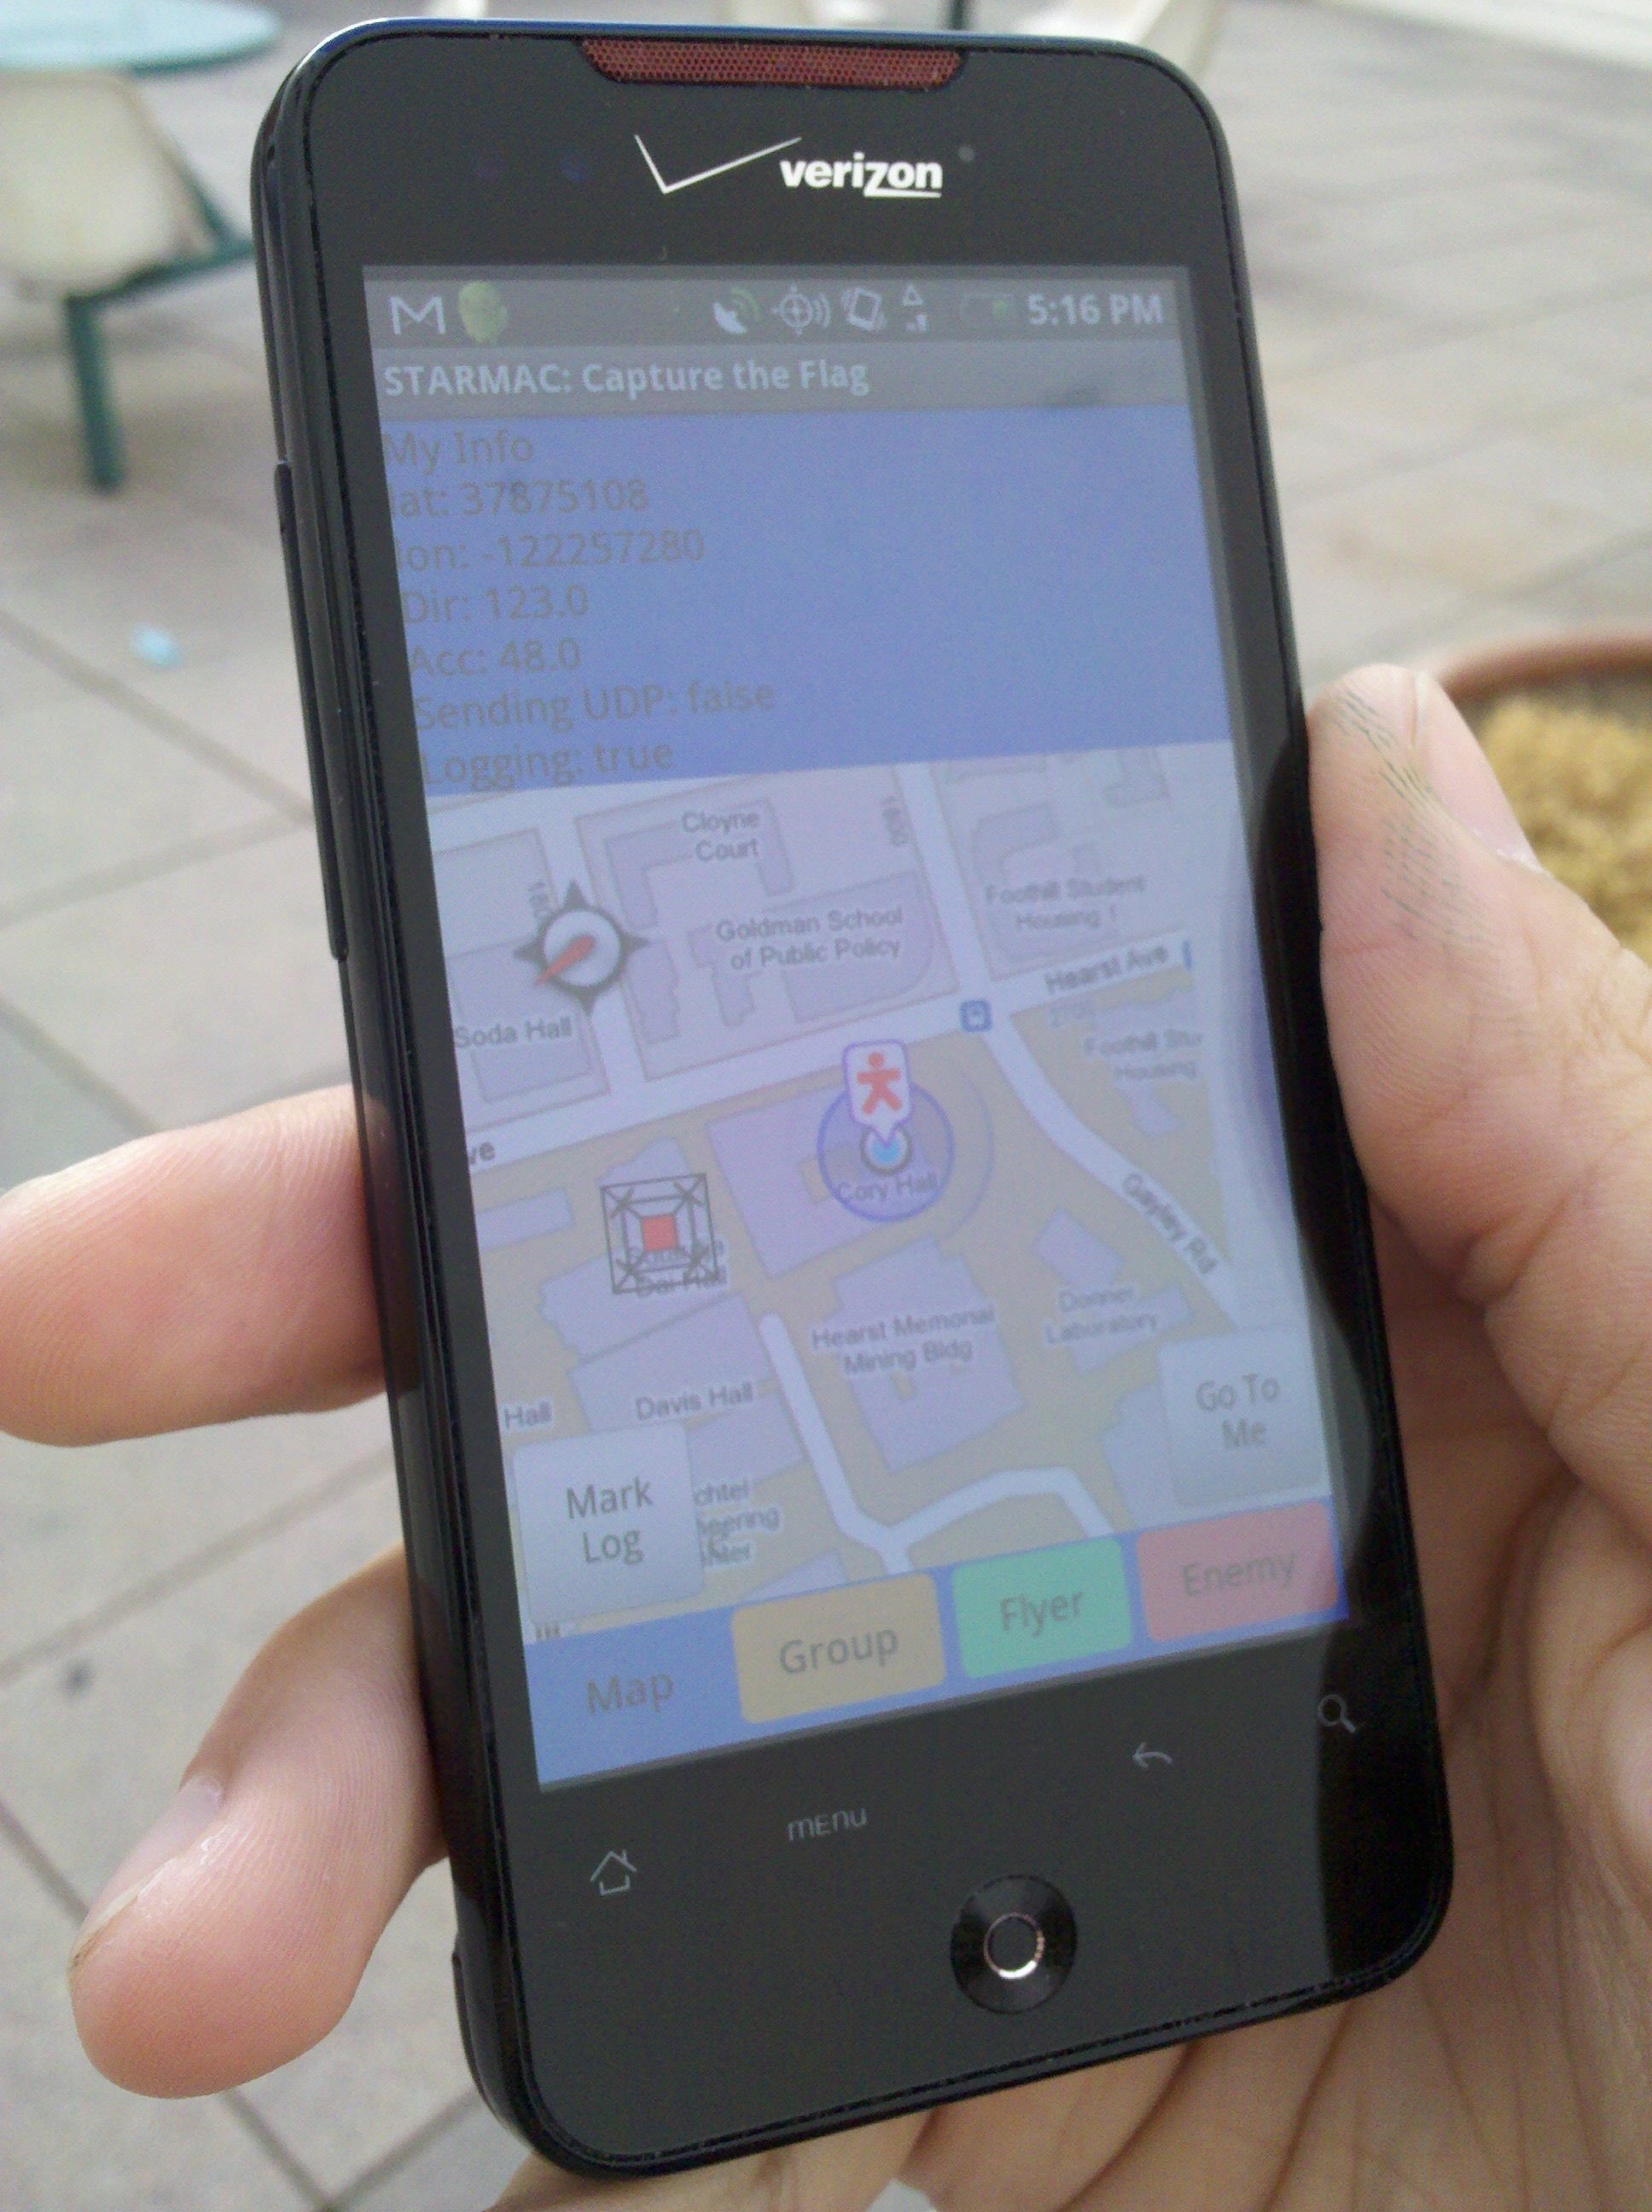
\includegraphics[width=0.38\linewidth]{figures/starmac_ctf_phone.jpg}  
\caption{\textbf{Smartphone application for playing automation-assisted capture-the-flag. }}
\label{fig:phoneGame}
\end{figure}

\section*{Acknowledgments}
The authors would like to thank Scott Hoag and Andrew Sy for their work on developing the capture-the-flag software.

%%%%%%%%%%%%%%%%%%%%%%%%%%%%%%%%%%%%%%%%%%%%%%%%%%%%%%%%%%%%%%%%%%%%%%%%%%%%%%%%

\vspace{-5mm}

\bibliographystyle{IEEEtran}
\bibliography{icra2011ctf}

\end{document}
